\documentclass{book}
\usepackage[a4paper,top=2.5cm,bottom=2.5cm,left=2.5cm,right=2.5cm]{geometry}
\usepackage{makeidx}
\usepackage{natbib}
\usepackage{graphicx}
\usepackage{multicol}
\usepackage{float}
\usepackage{listings}
\usepackage{color}
\usepackage{ifthen}
\usepackage[table]{xcolor}
\usepackage{textcomp}
\usepackage{alltt}
\usepackage{ifpdf}
\ifpdf
\usepackage[pdftex,
            pagebackref=true,
            colorlinks=true,
            linkcolor=blue,
            unicode
           ]{hyperref}
\else
\usepackage[ps2pdf,
            pagebackref=true,
            colorlinks=true,
            linkcolor=blue,
            unicode
           ]{hyperref}
\usepackage{pspicture}
\fi
\usepackage[utf8]{inputenc}
\usepackage{mathptmx}
\usepackage[scaled=.90]{helvet}
\usepackage{courier}
\usepackage{sectsty}
\usepackage{amssymb}
\usepackage[titles]{tocloft}
\usepackage{doxygen}
\lstset{language=C++,inputencoding=utf8,basicstyle=\footnotesize,breaklines=true,breakatwhitespace=true,tabsize=4,numbers=left }
\makeindex
\setcounter{tocdepth}{3}
\renewcommand{\footrulewidth}{0.4pt}
\renewcommand{\familydefault}{\sfdefault}
\hfuzz=15pt
\setlength{\emergencystretch}{15pt}
\hbadness=750
\tolerance=750
\begin{document}
\hypersetup{pageanchor=false,citecolor=blue}
\begin{titlepage}
\vspace*{7cm}
\begin{center}
{\Large My Project }\\
\vspace*{1cm}
{\large Generated by Doxygen 1.8.3.1}\\
\vspace*{0.5cm}
{\small Tue Dec 3 2013 02:19:11}\\
\end{center}
\end{titlepage}
\clearemptydoublepage
\pagenumbering{roman}
\tableofcontents
\clearemptydoublepage
\pagenumbering{arabic}
\hypersetup{pageanchor=true,citecolor=blue}
\chapter{Hierarchical Index}
\section{Class Hierarchy}
This inheritance list is sorted roughly, but not completely, alphabetically\-:\begin{DoxyCompactList}
\item \contentsline{section}{Barra\-Estado}{\pageref{classBarraEstado}}{}
\item \contentsline{section}{Box\-Opciones\-Basicas}{\pageref{classBoxOpcionesBasicas}}{}
\item \contentsline{section}{Celda}{\pageref{classCelda}}{}
\item \contentsline{section}{Columna}{\pageref{classColumna}}{}
\item \contentsline{section}{Info}{\pageref{classInfo}}{}
\item \contentsline{section}{Menu}{\pageref{classMenu}}{}
\item \contentsline{section}{Note\-Probabilidades}{\pageref{classNoteProbabilidades}}{}
\item \contentsline{section}{Persistidor}{\pageref{classPersistidor}}{}
\item \contentsline{section}{Probs}{\pageref{classProbs}}{}
\begin{DoxyCompactList}
\item \contentsline{section}{Prob\-Celdas}{\pageref{classProbCeldas}}{}
\item \contentsline{section}{Prob\-Columnas}{\pageref{classProbColumnas}}{}
\end{DoxyCompactList}
\item \contentsline{section}{Tablero}{\pageref{classTablero}}{}
\item Window\begin{DoxyCompactList}
\item \contentsline{section}{Main\-Window}{\pageref{classMainWindow}}{}
\end{DoxyCompactList}
\end{DoxyCompactList}

\chapter{Class Index}
\section{Class List}
Here are the classes, structs, unions and interfaces with brief descriptions\-:\begin{DoxyCompactList}
\item\contentsline{section}{\hyperlink{classBarraEstado}{Barra\-Estado} }{\pageref{classBarraEstado}}{}
\item\contentsline{section}{\hyperlink{classBoxOpcionesBasicas}{Box\-Opciones\-Basicas} }{\pageref{classBoxOpcionesBasicas}}{}
\item\contentsline{section}{\hyperlink{classCelda}{Celda} }{\pageref{classCelda}}{}
\item\contentsline{section}{\hyperlink{classColumna}{Columna} }{\pageref{classColumna}}{}
\item\contentsline{section}{\hyperlink{classInfo}{Info} }{\pageref{classInfo}}{}
\item\contentsline{section}{\hyperlink{classMainWindow}{Main\-Window} }{\pageref{classMainWindow}}{}
\item\contentsline{section}{\hyperlink{classMenu}{Menu} }{\pageref{classMenu}}{}
\item\contentsline{section}{\hyperlink{classNoteProbabilidades}{Note\-Probabilidades} }{\pageref{classNoteProbabilidades}}{}
\item\contentsline{section}{\hyperlink{classPersistidor}{Persistidor} }{\pageref{classPersistidor}}{}
\item\contentsline{section}{\hyperlink{classProbCeldas}{Prob\-Celdas} }{\pageref{classProbCeldas}}{}
\item\contentsline{section}{\hyperlink{classProbColumnas}{Prob\-Columnas} }{\pageref{classProbColumnas}}{}
\item\contentsline{section}{\hyperlink{classProbs}{Probs} }{\pageref{classProbs}}{}
\item\contentsline{section}{\hyperlink{classTablero}{Tablero} }{\pageref{classTablero}}{}
\end{DoxyCompactList}

\chapter{Class Documentation}
\hypertarget{classBarraEstado}{\section{Barra\-Estado Class Reference}
\label{classBarraEstado}\index{Barra\-Estado@{Barra\-Estado}}
}


{\ttfamily \#include $<$barraestado.\-h$>$}

\subsection*{Public Member Functions}
\begin{DoxyCompactItemize}
\item 
\hyperlink{classBarraEstado_a51d1e03ab0b7fb39c6d483ace492f4b2}{Barra\-Estado} (Glib\-::\-Ref\-Ptr$<$ Gtk\-::\-Builder $>$ \&builder)
\item 
void \hyperlink{classBarraEstado_a83e48331d4f0b0ddd1fd66c34cd248b7}{on\-Mostrar} (Gtk\-::\-Entry $\ast$entry\-Archivo)
\end{DoxyCompactItemize}


\subsection{Detailed Description}
Estatus bar para indicar mensajes de generacion de mapas. 

\subsection{Constructor \& Destructor Documentation}
\hypertarget{classBarraEstado_a51d1e03ab0b7fb39c6d483ace492f4b2}{\index{Barra\-Estado@{Barra\-Estado}!Barra\-Estado@{Barra\-Estado}}
\index{Barra\-Estado@{Barra\-Estado}!BarraEstado@{Barra\-Estado}}
\subsubsection[{Barra\-Estado}]{\setlength{\rightskip}{0pt plus 5cm}Barra\-Estado\-::\-Barra\-Estado (
\begin{DoxyParamCaption}
\item[{Glib\-::\-Ref\-Ptr$<$ Gtk\-::\-Builder $>$ \&}]{builder}
\end{DoxyParamCaption}
)\hspace{0.3cm}{\ttfamily [explicit]}}}\label{classBarraEstado_a51d1e03ab0b7fb39c6d483ace492f4b2}
Constructor del status bar usado para mostrar mensajes 
\begin{DoxyParams}{Parameters}
{\em builder\mbox{[}in\mbox{]},\-:} & Encargado de levantar el widget desde el archivo de glade. \\
\hline
\end{DoxyParams}


\subsection{Member Function Documentation}
\hypertarget{classBarraEstado_a83e48331d4f0b0ddd1fd66c34cd248b7}{\index{Barra\-Estado@{Barra\-Estado}!on\-Mostrar@{on\-Mostrar}}
\index{on\-Mostrar@{on\-Mostrar}!BarraEstado@{Barra\-Estado}}
\subsubsection[{on\-Mostrar}]{\setlength{\rightskip}{0pt plus 5cm}void Barra\-Estado\-::on\-Mostrar (
\begin{DoxyParamCaption}
\item[{Gtk\-::\-Entry $\ast$}]{entry\-Archivo}
\end{DoxyParamCaption}
)}}\label{classBarraEstado_a83e48331d4f0b0ddd1fd66c34cd248b7}
Muestra que mapa fue generado 
\begin{DoxyParams}{Parameters}
{\em entry\-Archivo\mbox{[}in\mbox{]},\-:} & Gtk\-::\-Entry contenedor del nombre del archivo generado. \\
\hline
\end{DoxyParams}


The documentation for this class was generated from the following files\-:\begin{DoxyCompactItemize}
\item 
barraestado.\-h\item 
barraestado.\-cpp\end{DoxyCompactItemize}

\hypertarget{classBoxOpcionesBasicas}{\section{Box\-Opciones\-Basicas Class Reference}
\label{classBoxOpcionesBasicas}\index{Box\-Opciones\-Basicas@{Box\-Opciones\-Basicas}}
}


{\ttfamily \#include $<$boxopcionesbasicas.\-h$>$}

\subsection*{Public Member Functions}
\begin{DoxyCompactItemize}
\item 
\hyperlink{classBoxOpcionesBasicas_a10d9db15b257fc95714511754206fb79}{Box\-Opciones\-Basicas} (Glib\-::\-Ref\-Ptr$<$ Gtk\-::\-Builder $>$ \&builder, \hyperlink{classTablero}{Tablero} $\ast$tablero)
\end{DoxyCompactItemize}
\subsection*{Public Attributes}
\begin{DoxyCompactItemize}
\item 
\hypertarget{classBoxOpcionesBasicas_ac75c6d189a34482d64b4909334f33e4d}{Glib\-::\-Ref\-Ptr$<$ Gtk\-::\-Adjustment $>$ {\bfseries adjustment\-\_\-cordx}}\label{classBoxOpcionesBasicas_ac75c6d189a34482d64b4909334f33e4d}

\item 
\hypertarget{classBoxOpcionesBasicas_a16a619543f0e8741edaf208180183a3d}{Glib\-::\-Ref\-Ptr$<$ Gtk\-::\-Adjustment $>$ {\bfseries adjustment\-\_\-cordy}}\label{classBoxOpcionesBasicas_a16a619543f0e8741edaf208180183a3d}

\item 
\hypertarget{classBoxOpcionesBasicas_a0fab1216f037c21255707ba4d9270968}{Glib\-::\-Ref\-Ptr$<$ Gtk\-::\-Adjustment $>$ {\bfseries adjustment\-\_\-nivel}}\label{classBoxOpcionesBasicas_a0fab1216f037c21255707ba4d9270968}

\end{DoxyCompactItemize}


\subsection{Detailed Description}
Panel izquierdo 

\subsection{Constructor \& Destructor Documentation}
\hypertarget{classBoxOpcionesBasicas_a10d9db15b257fc95714511754206fb79}{\index{Box\-Opciones\-Basicas@{Box\-Opciones\-Basicas}!Box\-Opciones\-Basicas@{Box\-Opciones\-Basicas}}
\index{Box\-Opciones\-Basicas@{Box\-Opciones\-Basicas}!BoxOpcionesBasicas@{Box\-Opciones\-Basicas}}
\subsubsection[{Box\-Opciones\-Basicas}]{\setlength{\rightskip}{0pt plus 5cm}Box\-Opciones\-Basicas\-::\-Box\-Opciones\-Basicas (
\begin{DoxyParamCaption}
\item[{Glib\-::\-Ref\-Ptr$<$ Gtk\-::\-Builder $>$ \&}]{builder, }
\item[{{\bf Tablero} $\ast$}]{tablero}
\end{DoxyParamCaption}
)}}\label{classBoxOpcionesBasicas_a10d9db15b257fc95714511754206fb79}
Constructor del panel izquierdo superior usado para la configuracion basica del nivel 
\begin{DoxyParams}{Parameters}
{\em builder\mbox{[}in\mbox{]},\-:} & Encargado de levantar el widget desde el archivo de glade. \\
\hline
\end{DoxyParams}


The documentation for this class was generated from the following files\-:\begin{DoxyCompactItemize}
\item 
boxopcionesbasicas.\-h\item 
boxopcionesbasicas.\-cpp\end{DoxyCompactItemize}

\hypertarget{classCelda}{\section{Celda Class Reference}
\label{classCelda}\index{Celda@{Celda}}
}


{\ttfamily \#include $<$celda.\-h$>$}

\subsection*{Public Member Functions}
\begin{DoxyCompactItemize}
\item 
\hypertarget{classCelda_a8062a01c45ec1a899c9c76238fe05e65}{{\bfseries Celda} (int x, int y)}\label{classCelda_a8062a01c45ec1a899c9c76238fe05e65}

\item 
\hypertarget{classCelda_a7a7d0b12316a5190a6c93efa1732c22c}{int {\bfseries get\-X} ()}\label{classCelda_a7a7d0b12316a5190a6c93efa1732c22c}

\item 
\hypertarget{classCelda_ae80269557d150404a44c87e8776d7c28}{int {\bfseries get\-Y} ()}\label{classCelda_ae80269557d150404a44c87e8776d7c28}

\item 
\hypertarget{classCelda_a6644d06c3166b158b099dd201cf31e9d}{\hyperlink{classInfo}{Info} $\ast$ {\bfseries get\-Info} ()}\label{classCelda_a6644d06c3166b158b099dd201cf31e9d}

\item 
\hypertarget{classCelda_aa51b9270362a5dbfddd26d63ce73640e}{void {\bfseries on\-\_\-adj\-\_\-changed} (Gtk\-::\-Spin\-Button $\ast$spinbutton, int id)}\label{classCelda_aa51b9270362a5dbfddd26d63ce73640e}

\item 
\hypertarget{classCelda_ada58827a0b78cedd93d252f5fb46270d}{void {\bfseries set\-Image} (const std\-::string \&file\-Name)}\label{classCelda_ada58827a0b78cedd93d252f5fb46270d}

\item 
\hypertarget{classCelda_a6215b4789f375d0dd51c2520ec4d0bf9}{void {\bfseries set\-Hueco} ()}\label{classCelda_a6215b4789f375d0dd51c2520ec4d0bf9}

\item 
\hypertarget{classCelda_aefde1dc1b85f037b4b3407047518a668}{bool {\bfseries is\-Hueco} ()}\label{classCelda_aefde1dc1b85f037b4b3407047518a668}

\item 
\hypertarget{classCelda_a8f8707d6810645d1790e97b73d7fae43}{std\-::string {\bfseries get\-Image} ()}\label{classCelda_a8f8707d6810645d1790e97b73d7fae43}

\end{DoxyCompactItemize}


\subsection{Detailed Description}
Representacion de cada casillero del tablero 

The documentation for this class was generated from the following files\-:\begin{DoxyCompactItemize}
\item 
celda.\-h\item 
celda.\-cpp\end{DoxyCompactItemize}

\hypertarget{classColumna}{\section{Columna Class Reference}
\label{classColumna}\index{Columna@{Columna}}
}


{\ttfamily \#include $<$columna.\-h$>$}

\subsection*{Public Member Functions}
\begin{DoxyCompactItemize}
\item 
\hyperlink{classColumna_a398754d5631668f97f75093594aa58da}{Columna} (int x, Gtk\-::\-Button $\ast$boton\-Columna)
\item 
void \hyperlink{classColumna_a70dbaf5ac0a963b5ec6a2e145eeced19}{on\-\_\-adj\-\_\-changed} (Gtk\-::\-Spin\-Button $\ast$spinbutton, int id)
\item 
\hypertarget{classColumna_a3fa57f60554cce389f05906443419f4f}{Gtk\-::\-Button $\ast$ {\bfseries get\-\_\-boton} ()}\label{classColumna_a3fa57f60554cce389f05906443419f4f}

\item 
\hypertarget{classColumna_a7f861f89db54fd07184eed4c6612ec6f}{\hyperlink{classInfo}{Info} $\ast$ {\bfseries get\-Info} ()}\label{classColumna_a7f861f89db54fd07184eed4c6612ec6f}

\end{DoxyCompactItemize}


\subsection{Detailed Description}
Entidad que modela las columnas para la aparicion de caramelos. 

\subsection{Constructor \& Destructor Documentation}
\hypertarget{classColumna_a398754d5631668f97f75093594aa58da}{\index{Columna@{Columna}!Columna@{Columna}}
\index{Columna@{Columna}!Columna@{Columna}}
\subsubsection[{Columna}]{\setlength{\rightskip}{0pt plus 5cm}Columna\-::\-Columna (
\begin{DoxyParamCaption}
\item[{int}]{x, }
\item[{Gtk\-::\-Button $\ast$}]{boton\-Columna}
\end{DoxyParamCaption}
)}}\label{classColumna_a398754d5631668f97f75093594aa58da}
Crea la columna x, que tenga el boton\-Columna activado. 
\begin{DoxyParams}{Parameters}
{\em x,\-:} & Numero de columna \\
\hline
{\em boton\-Columna,\-:} & Boton para activar la columna \\
\hline
\end{DoxyParams}


\subsection{Member Function Documentation}
\hypertarget{classColumna_a70dbaf5ac0a963b5ec6a2e145eeced19}{\index{Columna@{Columna}!on\-\_\-adj\-\_\-changed@{on\-\_\-adj\-\_\-changed}}
\index{on\-\_\-adj\-\_\-changed@{on\-\_\-adj\-\_\-changed}!Columna@{Columna}}
\subsubsection[{on\-\_\-adj\-\_\-changed}]{\setlength{\rightskip}{0pt plus 5cm}void Columna\-::on\-\_\-adj\-\_\-changed (
\begin{DoxyParamCaption}
\item[{Gtk\-::\-Spin\-Button $\ast$}]{spinbutton, }
\item[{int}]{id}
\end{DoxyParamCaption}
)}}\label{classColumna_a70dbaf5ac0a963b5ec6a2e145eeced19}
Cambia la probabilidad de la columna. 

The documentation for this class was generated from the following files\-:\begin{DoxyCompactItemize}
\item 
columna.\-h\item 
columna.\-cpp\end{DoxyCompactItemize}

\hypertarget{classInfo}{\section{Info Class Reference}
\label{classInfo}\index{Info@{Info}}
}


{\ttfamily \#include $<$info.\-h$>$}

\subsection*{Public Member Functions}
\begin{DoxyCompactItemize}
\item 
\hypertarget{classInfo_ad2a426dac2faca7998c6bcd2074baead}{void {\bfseries set\-Prob\-\_\-piezas} (int prob, int x)}\label{classInfo_ad2a426dac2faca7998c6bcd2074baead}

\item 
\hypertarget{classInfo_aa1536bee11bb5d2f9d76e2d44f26c6f5}{int {\bfseries get\-Prob\-\_\-piezas} (int idx)}\label{classInfo_aa1536bee11bb5d2f9d76e2d44f26c6f5}

\item 
\hypertarget{classInfo_a673f62e1f79094f22bf7ef0656ba38f3}{int $\ast$ {\bfseries get\-Array} ()}\label{classInfo_a673f62e1f79094f22bf7ef0656ba38f3}

\end{DoxyCompactItemize}


\subsection{Detailed Description}
Clase para modelar las probabilidades 

The documentation for this class was generated from the following files\-:\begin{DoxyCompactItemize}
\item 
info.\-h\item 
info.\-cpp\end{DoxyCompactItemize}

\hypertarget{classMainWindow}{\section{Main\-Window Class Reference}
\label{classMainWindow}\index{Main\-Window@{Main\-Window}}
}


{\ttfamily \#include $<$cliente.\-main\-\_\-window.\-h$>$}

Inheritance diagram for Main\-Window\-:\begin{figure}[H]
\begin{center}
\leavevmode
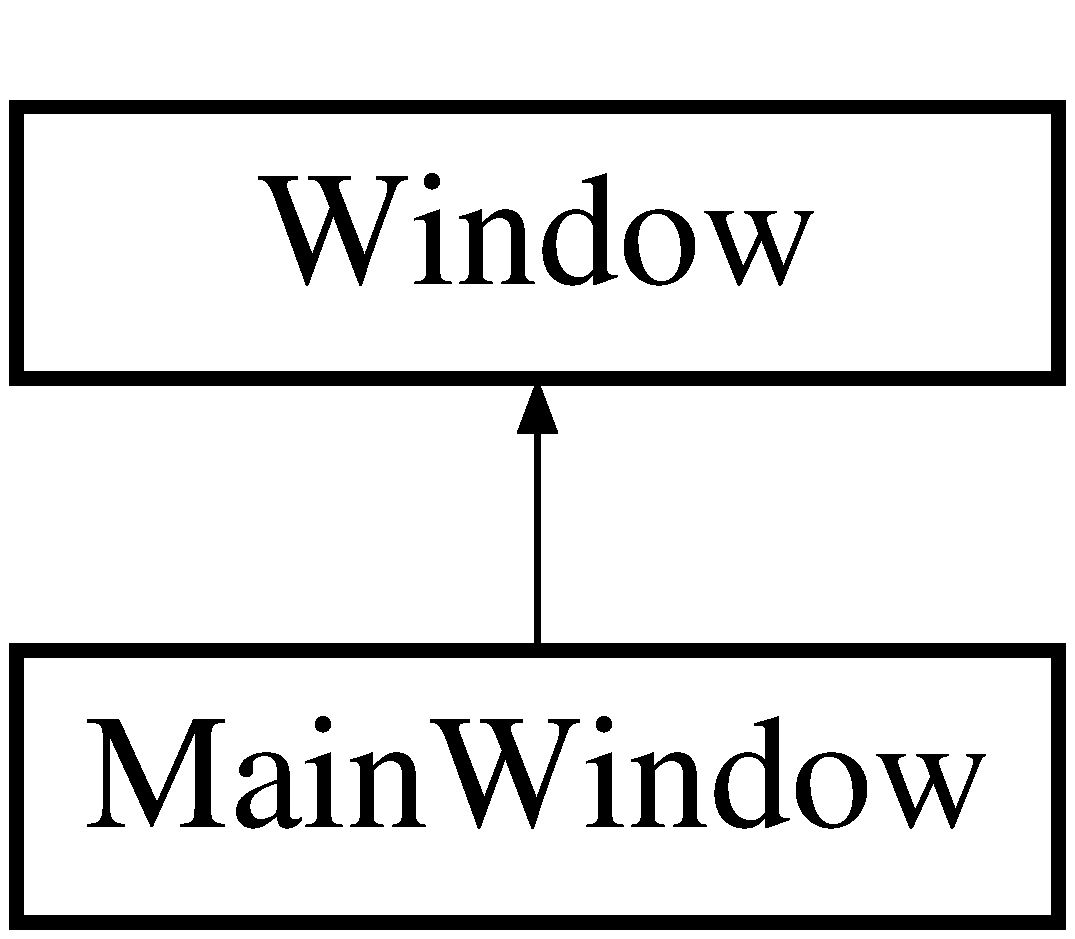
\includegraphics[height=3.000000cm]{classMainWindow}
\end{center}
\end{figure}
\subsection*{Public Member Functions}
\begin{DoxyCompactItemize}
\item 
\hypertarget{classMainWindow_a5a199f2a565bea157bf757965231009b}{void {\bfseries set\-Text} (std\-::string \&str)}\label{classMainWindow_a5a199f2a565bea157bf757965231009b}

\item 
virtual void \hyperlink{classMainWindow_a735c7caa0682694dc016f8bb80ef1f8c}{mensaje} (Json\-::\-Value \&data)
\end{DoxyCompactItemize}
\subsection*{Protected Member Functions}
\begin{DoxyCompactItemize}
\item 
\hypertarget{classMainWindow_a84f1debb16a5d9433115085502664ff1}{void {\bfseries on\-List\-Games} (int code, Json\-::\-Value \&data)}\label{classMainWindow_a84f1debb16a5d9433115085502664ff1}

\item 
\hypertarget{classMainWindow_af1f2f2aa17dcf3f727dca0935e0f9903}{void {\bfseries on\-List\-Maps} (int code, Json\-::\-Value \&data)}\label{classMainWindow_af1f2f2aa17dcf3f727dca0935e0f9903}

\item 
\hypertarget{classMainWindow_a67675f346522095602ef474d1d4a5168}{void {\bfseries on\-\_\-partidas} ()}\label{classMainWindow_a67675f346522095602ef474d1d4a5168}

\item 
\hypertarget{classMainWindow_a9d05b4619e7e5424768cca963922968e}{void {\bfseries join\-\_\-partidas} ()}\label{classMainWindow_a9d05b4619e7e5424768cca963922968e}

\item 
\hypertarget{classMainWindow_a3a1541637c02219b285d5bf9bc6381a1}{void {\bfseries on\-\_\-mapas} ()}\label{classMainWindow_a3a1541637c02219b285d5bf9bc6381a1}

\item 
\hypertarget{classMainWindow_a42724db9575b3be2f1a734351ab51262}{void {\bfseries on\-\_\-crear\-\_\-partida} ()}\label{classMainWindow_a42724db9575b3be2f1a734351ab51262}

\item 
\hypertarget{classMainWindow_acc25dd6bdbfdf9d4cf04c4a099b00e54}{virtual bool {\bfseries on\-Close} ()}\label{classMainWindow_acc25dd6bdbfdf9d4cf04c4a099b00e54}

\end{DoxyCompactItemize}
\subsection*{Protected Attributes}
\begin{DoxyCompactItemize}
\item 
\hypertarget{classMainWindow_adc5c31aa7147c5273128a37c61531935}{Menu\-Bar\-Disconnect {\bfseries menubar}}\label{classMainWindow_adc5c31aa7147c5273128a37c61531935}

\item 
\hypertarget{classMainWindow_a528b74e7fb62a056c7db7e4cc3405f0e}{Gtk\-::\-Notebook {\bfseries tabs}}\label{classMainWindow_a528b74e7fb62a056c7db7e4cc3405f0e}

\item 
\hypertarget{classMainWindow_a3f6985d785f060685e1cd28526fa7f03}{Gtk\-::\-Label {\bfseries label\-Partidas}}\label{classMainWindow_a3f6985d785f060685e1cd28526fa7f03}

\item 
\hypertarget{classMainWindow_a07cf47f1cb3a6fe3e533390db18b9040}{Gtk\-::\-V\-Box {\bfseries m\-\_\-\-V\-Box\-\_\-partidas}}\label{classMainWindow_a07cf47f1cb3a6fe3e533390db18b9040}

\item 
\hypertarget{classMainWindow_ac6f0abacd5af95429201d40b4ec9ca95}{Gtk\-::\-H\-Box {\bfseries m\-\_\-\-H\-Box\-\_\-partidas\-\_\-buttons}}\label{classMainWindow_ac6f0abacd5af95429201d40b4ec9ca95}

\item 
\hypertarget{classMainWindow_ad6a19e7c9f49905bd7bc0c25a1cd50f2}{Gtk\-::\-Button {\bfseries button\-\_\-partidas\-\_\-act}}\label{classMainWindow_ad6a19e7c9f49905bd7bc0c25a1cd50f2}

\item 
\hypertarget{classMainWindow_a1af69f7c49665084fb746433fb7e6fd3}{Gtk\-::\-Button {\bfseries button\-\_\-partidas\-\_\-con}}\label{classMainWindow_a1af69f7c49665084fb746433fb7e6fd3}

\item 
\hypertarget{classMainWindow_a395e40c010bd07252453e9adc64faeb4}{Gtk\-::\-Scrolled\-Window {\bfseries m\-\_\-\-Scrolled\-Partidas}}\label{classMainWindow_a395e40c010bd07252453e9adc64faeb4}

\item 
\hypertarget{classMainWindow_a37807219b285408f8d30efe28a822e62}{Lista\-Partidas {\bfseries m\-\_\-\-Tree\-View}}\label{classMainWindow_a37807219b285408f8d30efe28a822e62}

\item 
\hypertarget{classMainWindow_ae037e61673e84e41a6f28975dd730fd4}{Gtk\-::\-Label {\bfseries label\-Mapas}}\label{classMainWindow_ae037e61673e84e41a6f28975dd730fd4}

\item 
\hypertarget{classMainWindow_a60812cc8e7aa530e73ea1f6515eb7acb}{Gtk\-::\-V\-Box {\bfseries m\-\_\-\-V\-Box\-\_\-mapas}}\label{classMainWindow_a60812cc8e7aa530e73ea1f6515eb7acb}

\item 
\hypertarget{classMainWindow_ab04dad89a39bd6a05ab9b360ca301544}{Gtk\-::\-H\-Box {\bfseries m\-\_\-\-H\-Box\-\_\-mapas\-\_\-buttons}}\label{classMainWindow_ab04dad89a39bd6a05ab9b360ca301544}

\item 
\hypertarget{classMainWindow_ab2355dd68ee5c74d391062fa873ad826}{Gtk\-::\-Button {\bfseries button\-\_\-mapas\-\_\-act}}\label{classMainWindow_ab2355dd68ee5c74d391062fa873ad826}

\item 
\hypertarget{classMainWindow_afc9a680bd1aa98e092db560b592c4467}{Gtk\-::\-Button {\bfseries button\-\_\-mapas\-\_\-cre}}\label{classMainWindow_afc9a680bd1aa98e092db560b592c4467}

\item 
\hypertarget{classMainWindow_a8048011e7fd4242ec20a1a5756ad5bf3}{Gtk\-::\-Scrolled\-Window {\bfseries m\-\_\-\-Scrolled\-Mapas}}\label{classMainWindow_a8048011e7fd4242ec20a1a5756ad5bf3}

\item 
\hypertarget{classMainWindow_a978da20f46529029b3ff46b246fcee09}{Lista\-Mapas {\bfseries m\-\_\-\-Tree\-View\-Mapas}}\label{classMainWindow_a978da20f46529029b3ff46b246fcee09}

\item 
\hypertarget{classMainWindow_a6f9f64b3e9d8baef03dc65513cb68530}{Gtk\-::\-V\-Box {\bfseries main\-V}}\label{classMainWindow_a6f9f64b3e9d8baef03dc65513cb68530}

\item 
\hypertarget{classMainWindow_a7d222c50fa848d67546c7f212875f4c1}{Gtk\-::\-H\-Box {\bfseries tab\-Box}}\label{classMainWindow_a7d222c50fa848d67546c7f212875f4c1}

\item 
\hypertarget{classMainWindow_abe645ed1d8d45e5ba978f324c29d7e09}{Gtk\-::\-Label {\bfseries status\-Label}}\label{classMainWindow_abe645ed1d8d45e5ba978f324c29d7e09}

\end{DoxyCompactItemize}
\subsection*{Additional Inherited Members}


\subsection{Detailed Description}
Ventana de Seleccionar y/o crear partida 

\subsection{Member Function Documentation}
\hypertarget{classMainWindow_a735c7caa0682694dc016f8bb80ef1f8c}{\index{Main\-Window@{Main\-Window}!mensaje@{mensaje}}
\index{mensaje@{mensaje}!MainWindow@{Main\-Window}}
\subsubsection[{mensaje}]{\setlength{\rightskip}{0pt plus 5cm}void Main\-Window\-::mensaje (
\begin{DoxyParamCaption}
\item[{Json\-::\-Value \&}]{data}
\end{DoxyParamCaption}
)\hspace{0.3cm}{\ttfamily [virtual]}}}\label{classMainWindow_a735c7caa0682694dc016f8bb80ef1f8c}
Metodo que reciben los mensajes del servidor, que deben mostrar. 

Implements \hyperlink{classWindow_a6034ea4f54b6647de07b19ff95fb22ae}{Window}.



The documentation for this class was generated from the following files\-:\begin{DoxyCompactItemize}
\item 
cliente.\-main\-\_\-window.\-h\item 
cliente.\-main\-\_\-window.\-cpp\end{DoxyCompactItemize}

\hypertarget{classMenu}{\section{Menu Class Reference}
\label{classMenu}\index{Menu@{Menu}}
}


{\ttfamily \#include $<$menu.\-h$>$}

\subsection*{Public Member Functions}
\begin{DoxyCompactItemize}
\item 
\hypertarget{classMenu_a251f653c4eec0db5f8b44a3f2ac79484}{{\bfseries Menu} (Glib\-::\-Ref\-Ptr$<$ Gtk\-::\-Builder $>$ \&builder)}\label{classMenu_a251f653c4eec0db5f8b44a3f2ac79484}

\end{DoxyCompactItemize}


\subsection{Detailed Description}
\hyperlink{classMenu}{Menu} superior con las opciones de salir, about y help 

The documentation for this class was generated from the following files\-:\begin{DoxyCompactItemize}
\item 
menu.\-h\item 
menu.\-cpp\end{DoxyCompactItemize}

\hypertarget{classNoteProbabilidades}{\section{Note\-Probabilidades Class Reference}
\label{classNoteProbabilidades}\index{Note\-Probabilidades@{Note\-Probabilidades}}
}


{\ttfamily \#include $<$noteprobabilidades.\-h$>$}

\subsection*{Public Member Functions}
\begin{DoxyCompactItemize}
\item 
\hypertarget{classNoteProbabilidades_a0cf18f353a4443bca5f797781cc2ea8a}{{\bfseries Note\-Probabilidades} (Glib\-::\-Ref\-Ptr$<$ Gtk\-::\-Builder $>$ \&builder, \hyperlink{classTablero}{Tablero} $\ast$tablero)}\label{classNoteProbabilidades_a0cf18f353a4443bca5f797781cc2ea8a}

\end{DoxyCompactItemize}


\subsection{Detailed Description}
Clase contenedora de las probabilidades de celda y columna dentro del notebook de probabilidades. 

The documentation for this class was generated from the following files\-:\begin{DoxyCompactItemize}
\item 
noteprobabilidades.\-h\item 
noteprobabilidades.\-cpp\end{DoxyCompactItemize}

\hypertarget{classPersistidor}{\section{Persistidor Class Reference}
\label{classPersistidor}\index{Persistidor@{Persistidor}}
}


{\ttfamily \#include $<$persistidor.\-h$>$}

\subsection*{Static Public Member Functions}
\begin{DoxyCompactItemize}
\item 
static void \hyperlink{classPersistidor_a2a446a5a35c9328bebc0d471efc62138}{persistir} (Json\-::\-Value \&nivel, const std\-::string \&nombre)
\end{DoxyCompactItemize}


\subsection{Detailed Description}
Clase encargada de volcar la informacion de los mapas a un archivo 

\subsection{Member Function Documentation}
\hypertarget{classPersistidor_a2a446a5a35c9328bebc0d471efc62138}{\index{Persistidor@{Persistidor}!persistir@{persistir}}
\index{persistir@{persistir}!Persistidor@{Persistidor}}
\subsubsection[{persistir}]{\setlength{\rightskip}{0pt plus 5cm}static void Persistidor\-::persistir (
\begin{DoxyParamCaption}
\item[{Json\-::\-Value \&}]{nivel, }
\item[{const std\-::string \&}]{nombre}
\end{DoxyParamCaption}
)\hspace{0.3cm}{\ttfamily [inline]}, {\ttfamily [static]}}}\label{classPersistidor_a2a446a5a35c9328bebc0d471efc62138}
Persiste el mapa. 
\begin{DoxyParams}{Parameters}
{\em nivel,\-:} & Nivel a persistir. \\
\hline
{\em nombre,\-:} & Nombre del mapa a persistir. \\
\hline
\end{DoxyParams}


The documentation for this class was generated from the following file\-:\begin{DoxyCompactItemize}
\item 
persistidor.\-h\end{DoxyCompactItemize}

\hypertarget{classProbCeldas}{\section{Prob\-Celdas Class Reference}
\label{classProbCeldas}\index{Prob\-Celdas@{Prob\-Celdas}}
}


{\ttfamily \#include $<$probceldas.\-h$>$}

Inheritance diagram for Prob\-Celdas\-:\begin{figure}[H]
\begin{center}
\leavevmode
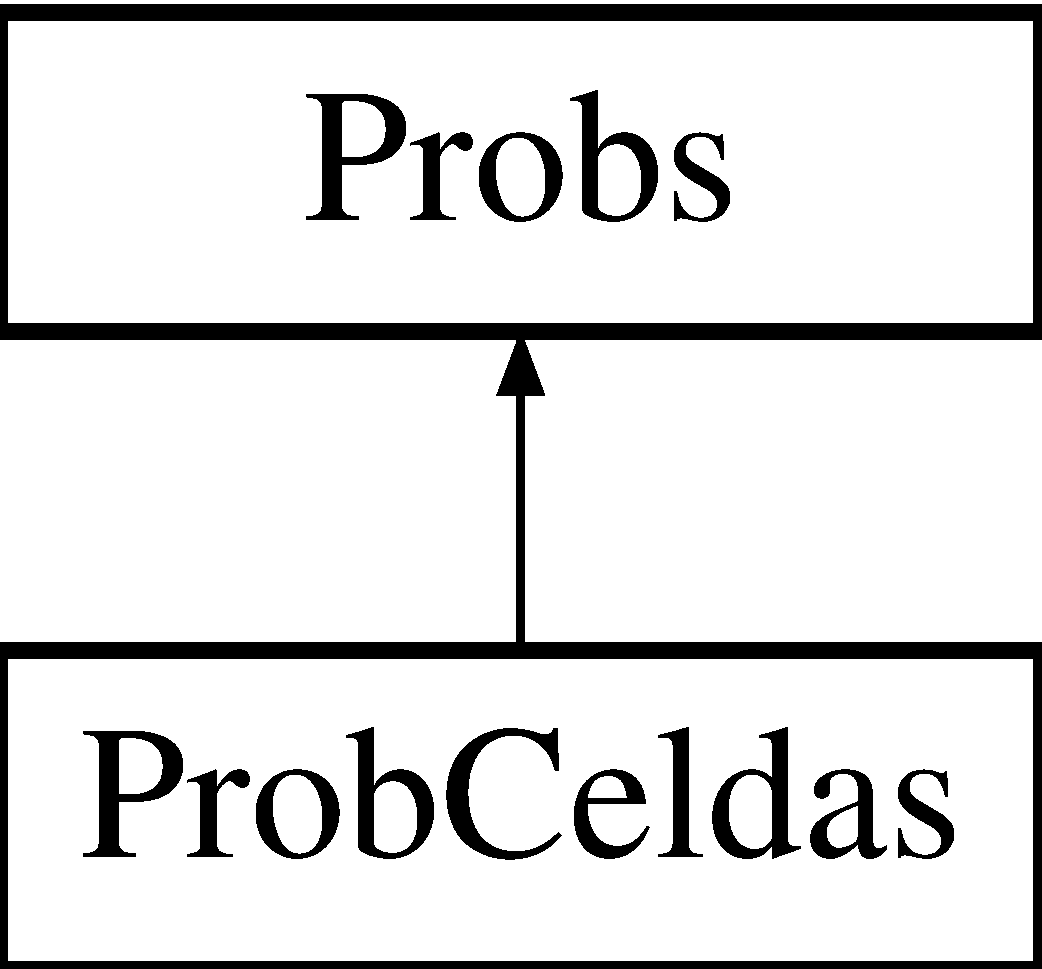
\includegraphics[height=2.000000cm]{classProbCeldas}
\end{center}
\end{figure}
\subsection*{Public Member Functions}
\begin{DoxyCompactItemize}
\item 
\hyperlink{classProbCeldas_aad40cbe3d82f9c0a2a2cf92fff3bf80b}{Prob\-Celdas} (\hyperlink{classTablero}{Tablero} $\ast$tablero, Glib\-::\-Ref\-Ptr$<$ Gtk\-::\-Builder $>$ \&builder)
\end{DoxyCompactItemize}
\subsection*{Additional Inherited Members}


\subsection{Detailed Description}
Clase contenedora de las opciones de la celda 

\subsection{Constructor \& Destructor Documentation}
\hypertarget{classProbCeldas_aad40cbe3d82f9c0a2a2cf92fff3bf80b}{\index{Prob\-Celdas@{Prob\-Celdas}!Prob\-Celdas@{Prob\-Celdas}}
\index{Prob\-Celdas@{Prob\-Celdas}!ProbCeldas@{Prob\-Celdas}}
\subsubsection[{Prob\-Celdas}]{\setlength{\rightskip}{0pt plus 5cm}Prob\-Celdas\-::\-Prob\-Celdas (
\begin{DoxyParamCaption}
\item[{{\bf Tablero} $\ast$}]{tablero, }
\item[{Glib\-::\-Ref\-Ptr$<$ Gtk\-::\-Builder $>$ \&}]{builder}
\end{DoxyParamCaption}
)}}\label{classProbCeldas_aad40cbe3d82f9c0a2a2cf92fff3bf80b}
Se crea el frame con un filechooser, un boton para el hueco y se conectan los spinbuttons. 

The documentation for this class was generated from the following files\-:\begin{DoxyCompactItemize}
\item 
probceldas.\-h\item 
probceldas.\-cpp\end{DoxyCompactItemize}

\hypertarget{classProbColumnas}{\section{Prob\-Columnas Class Reference}
\label{classProbColumnas}\index{Prob\-Columnas@{Prob\-Columnas}}
}
Inheritance diagram for Prob\-Columnas\-:\begin{figure}[H]
\begin{center}
\leavevmode
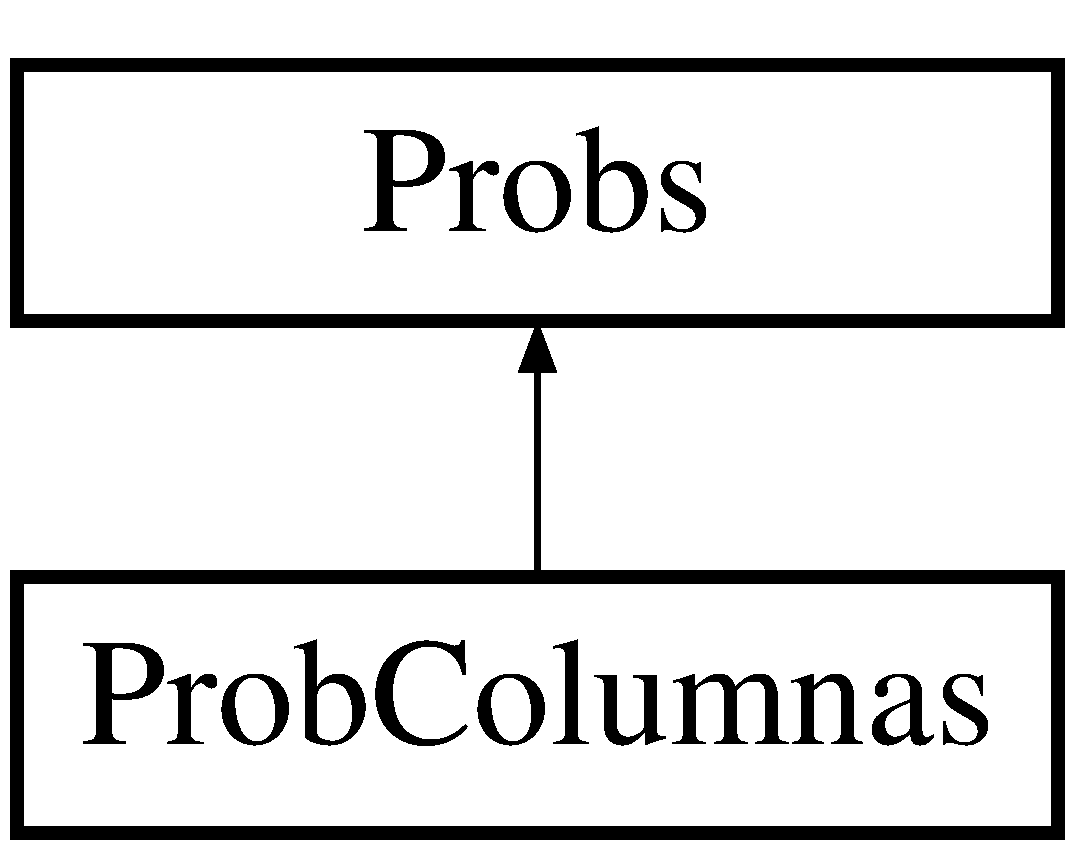
\includegraphics[height=2.000000cm]{classProbColumnas}
\end{center}
\end{figure}
\subsection*{Public Member Functions}
\begin{DoxyCompactItemize}
\item 
\hypertarget{classProbColumnas_a660c108a2f78121c8dce6a406af268ea}{{\bfseries Prob\-Columnas} (\hyperlink{classTablero}{Tablero} $\ast$tablero, Glib\-::\-Ref\-Ptr$<$ Gtk\-::\-Builder $>$ \&builder)}\label{classProbColumnas_a660c108a2f78121c8dce6a406af268ea}

\end{DoxyCompactItemize}
\subsection*{Additional Inherited Members}


The documentation for this class was generated from the following files\-:\begin{DoxyCompactItemize}
\item 
probcolumnas.\-h\item 
probcolumnas.\-cpp\end{DoxyCompactItemize}

\hypertarget{classProbs}{\section{Probs Class Reference}
\label{classProbs}\index{Probs@{Probs}}
}


{\ttfamily \#include $<$generalprobs.\-h$>$}

Inheritance diagram for Probs\-:\begin{figure}[H]
\begin{center}
\leavevmode
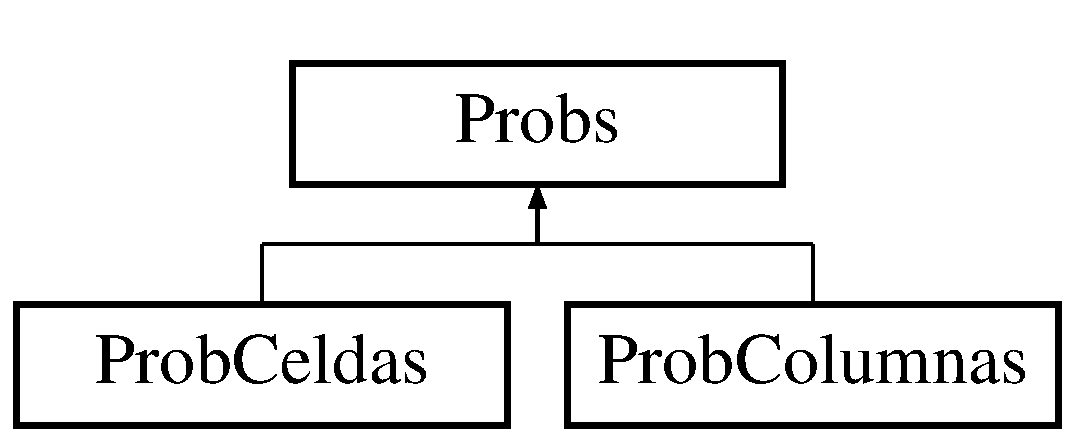
\includegraphics[height=2.000000cm]{classProbs}
\end{center}
\end{figure}
\subsection*{Public Member Functions}
\begin{DoxyCompactItemize}
\item 
\hypertarget{classProbs_ae64395229e694c15a5167cb99625bcf2}{{\bfseries Probs} (\hyperlink{classTablero}{Tablero} $\ast$tablero, Glib\-::\-Ref\-Ptr$<$ Gtk\-::\-Builder $>$ \&builder, int start\-Number, int final\-Number, std\-::string frame\-Name)}\label{classProbs_ae64395229e694c15a5167cb99625bcf2}

\end{DoxyCompactItemize}
\subsection*{Protected Member Functions}
\begin{DoxyCompactItemize}
\item 
\hypertarget{classProbs_a8749c6a4f39c23c92ed522ac22fe4e26}{void {\bfseries cargar\-Botones} (Glib\-::\-Ref\-Ptr$<$ Gtk\-::\-Builder $>$ \&builder, int firstbutton, int lastbutton)}\label{classProbs_a8749c6a4f39c23c92ed522ac22fe4e26}

\end{DoxyCompactItemize}
\subsection*{Protected Attributes}
\begin{DoxyCompactItemize}
\item 
\hypertarget{classProbs_ac5d2405551d7aaa74920356b09e1de1e}{\hyperlink{classTablero}{Tablero} $\ast$ {\bfseries tablero}}\label{classProbs_ac5d2405551d7aaa74920356b09e1de1e}

\item 
\hypertarget{classProbs_a9a02b4a3aee0e9bc42ed626b232de5d3}{std\-::vector$<$ Gtk\-::\-Spin\-Button $\ast$ $>$ {\bfseries spinbuttons}}\label{classProbs_a9a02b4a3aee0e9bc42ed626b232de5d3}

\item 
\hypertarget{classProbs_ae5a188ea47bbe0160cc80a3ba3fda2a7}{std\-::vector$<$ Glib\-::\-Ref\-Ptr\\*
$<$ Gtk\-::\-Adjustment $>$ $>$ {\bfseries adjustments}}\label{classProbs_ae5a188ea47bbe0160cc80a3ba3fda2a7}

\end{DoxyCompactItemize}


\subsection{Detailed Description}
Clase abstracta para el manejo de probabilidades de celda y columna 

The documentation for this class was generated from the following files\-:\begin{DoxyCompactItemize}
\item 
generalprobs.\-h\item 
generalprobs.\-cpp\end{DoxyCompactItemize}

\hypertarget{classTablero}{\section{Tablero Class Reference}
\label{classTablero}\index{Tablero@{Tablero}}
}


{\ttfamily \#include $<$tablero.\-h$>$}

\subsection*{Public Types}
\begin{DoxyCompactItemize}
\item 
typedef sigc\-::signal$<$ void $>$ \hyperlink{classTablero_a1c847f6d745139e22ca87a32f82ded14}{type\-\_\-signal\-\_\-uncheck}
\end{DoxyCompactItemize}
\subsection*{Public Member Functions}
\begin{DoxyCompactItemize}
\item 
\hyperlink{classTablero_ada8ba5e6781488793f2f78c3799aa4ff}{Tablero} (Glib\-::\-Ref\-Ptr$<$ Gtk\-::\-Builder $>$ \&builder)
\item 
void \hyperlink{classTablero_a58e80bae3f019987b9283723f8a57b84}{on\-\_\-adj\-Cols\-\_\-changed\-\_\-tablero} (Gtk\-::\-Spin\-Button $\ast$spinbutton, int id)
\item 
void \hyperlink{classTablero_afacc7a7dd1f42590e39b87cae48e3275}{on\-\_\-cordx\-\_\-changed} (Gtk\-::\-Spin\-Button $\ast$spin\-\_\-x)
\item 
void \hyperlink{classTablero_a2e94fb8a39b63af67fc1d2d00eb40bb3}{on\-\_\-cordy\-\_\-changed} (Gtk\-::\-Spin\-Button $\ast$spin\-\_\-y)
\item 
void \hyperlink{classTablero_ab7f1519be16814243a5b425600dd59a0}{on\-\_\-adj\-\_\-changed\-\_\-tablero} (Gtk\-::\-Spin\-Button $\ast$spinbutton, int id)
\item 
void \hyperlink{classTablero_acdc841e43131788e8d722f341d2df174}{on\-\_\-image\-\_\-changed\-\_\-tablero} (Gtk\-::\-File\-Chooser $\ast$file\-Chooser)
\item 
void \hyperlink{classTablero_a910b04b2d9807d8618b2e176942da950}{on\-\_\-image\-\_\-fondo\-\_\-changed\-\_\-tablero} (Gtk\-::\-File\-Chooser $\ast$file\-Chooser)
\item 
void \hyperlink{classTablero_a2e329c07dbc1a33793958eb8b192bbc3}{on\-\_\-check\-\_\-button\-\_\-tablero} ()
\item 
void \hyperlink{classTablero_a17f4eadec115ef30e08a45d9b26a6fc4}{json\-Celdas} (Json\-::\-Value \&nivel, const std\-::string \&nombre)
\item 
void \hyperlink{classTablero_a47c278b608b5e1dd22aeafcdba0ea0f2}{json\-Columnas} (Json\-::\-Value \&nivel, const std\-::string \&nombre)
\item 
\hypertarget{classTablero_aefdae69f836627a44aec877940919099}{\hyperlink{classTablero_a1c847f6d745139e22ca87a32f82ded14}{type\-\_\-signal\-\_\-uncheck} {\bfseries signal\-\_\-uncheck} ()}\label{classTablero_aefdae69f836627a44aec877940919099}

\end{DoxyCompactItemize}


\subsection{Detailed Description}
\hyperlink{classTablero}{Tablero} de juego . 

\subsection{Member Typedef Documentation}
\hypertarget{classTablero_a1c847f6d745139e22ca87a32f82ded14}{\index{Tablero@{Tablero}!type\-\_\-signal\-\_\-uncheck@{type\-\_\-signal\-\_\-uncheck}}
\index{type\-\_\-signal\-\_\-uncheck@{type\-\_\-signal\-\_\-uncheck}!Tablero@{Tablero}}
\subsubsection[{type\-\_\-signal\-\_\-uncheck}]{\setlength{\rightskip}{0pt plus 5cm}typedef sigc\-::signal$<$ void $>$ {\bf Tablero\-::type\-\_\-signal\-\_\-uncheck}}}\label{classTablero_a1c847f6d745139e22ca87a32f82ded14}
Senal que se emite despues de hacer click 

\subsection{Constructor \& Destructor Documentation}
\hypertarget{classTablero_ada8ba5e6781488793f2f78c3799aa4ff}{\index{Tablero@{Tablero}!Tablero@{Tablero}}
\index{Tablero@{Tablero}!Tablero@{Tablero}}
\subsubsection[{Tablero}]{\setlength{\rightskip}{0pt plus 5cm}Tablero\-::\-Tablero (
\begin{DoxyParamCaption}
\item[{Glib\-::\-Ref\-Ptr$<$ Gtk\-::\-Builder $>$ \&}]{builder}
\end{DoxyParamCaption}
)\hspace{0.3cm}{\ttfamily [explicit]}}}\label{classTablero_ada8ba5e6781488793f2f78c3799aa4ff}
Constructor de tablero. 
\begin{DoxyParams}{Parameters}
{\em builder,\-:} & Utilizado para levantar widgets del archivo de glade \\
\hline
\end{DoxyParams}


\subsection{Member Function Documentation}
\hypertarget{classTablero_a17f4eadec115ef30e08a45d9b26a6fc4}{\index{Tablero@{Tablero}!json\-Celdas@{json\-Celdas}}
\index{json\-Celdas@{json\-Celdas}!Tablero@{Tablero}}
\subsubsection[{json\-Celdas}]{\setlength{\rightskip}{0pt plus 5cm}void Tablero\-::json\-Celdas (
\begin{DoxyParamCaption}
\item[{Json\-::\-Value \&}]{nivel, }
\item[{const std\-::string \&}]{nombre}
\end{DoxyParamCaption}
)}}\label{classTablero_a17f4eadec115ef30e08a45d9b26a6fc4}
Serializa la informacion de las celdas. \hypertarget{classTablero_a47c278b608b5e1dd22aeafcdba0ea0f2}{\index{Tablero@{Tablero}!json\-Columnas@{json\-Columnas}}
\index{json\-Columnas@{json\-Columnas}!Tablero@{Tablero}}
\subsubsection[{json\-Columnas}]{\setlength{\rightskip}{0pt plus 5cm}void Tablero\-::json\-Columnas (
\begin{DoxyParamCaption}
\item[{Json\-::\-Value \&}]{nivel, }
\item[{const std\-::string \&}]{nombre}
\end{DoxyParamCaption}
)}}\label{classTablero_a47c278b608b5e1dd22aeafcdba0ea0f2}
Serializa la informacion de las celdas. \hypertarget{classTablero_ab7f1519be16814243a5b425600dd59a0}{\index{Tablero@{Tablero}!on\-\_\-adj\-\_\-changed\-\_\-tablero@{on\-\_\-adj\-\_\-changed\-\_\-tablero}}
\index{on\-\_\-adj\-\_\-changed\-\_\-tablero@{on\-\_\-adj\-\_\-changed\-\_\-tablero}!Tablero@{Tablero}}
\subsubsection[{on\-\_\-adj\-\_\-changed\-\_\-tablero}]{\setlength{\rightskip}{0pt plus 5cm}void Tablero\-::on\-\_\-adj\-\_\-changed\-\_\-tablero (
\begin{DoxyParamCaption}
\item[{Gtk\-::\-Spin\-Button $\ast$}]{spinbutton, }
\item[{int}]{id}
\end{DoxyParamCaption}
)}}\label{classTablero_ab7f1519be16814243a5b425600dd59a0}
Se encarga de poner probabilidades por celda. 
\begin{DoxyParams}{Parameters}
{\em spinbutton,\-:} & Spin\-Button que cambio. \\
\hline
{\em id,\-:} & Numero de Spin\-Button que cambio. \\
\hline
\end{DoxyParams}
\hypertarget{classTablero_a58e80bae3f019987b9283723f8a57b84}{\index{Tablero@{Tablero}!on\-\_\-adj\-Cols\-\_\-changed\-\_\-tablero@{on\-\_\-adj\-Cols\-\_\-changed\-\_\-tablero}}
\index{on\-\_\-adj\-Cols\-\_\-changed\-\_\-tablero@{on\-\_\-adj\-Cols\-\_\-changed\-\_\-tablero}!Tablero@{Tablero}}
\subsubsection[{on\-\_\-adj\-Cols\-\_\-changed\-\_\-tablero}]{\setlength{\rightskip}{0pt plus 5cm}void Tablero\-::on\-\_\-adj\-Cols\-\_\-changed\-\_\-tablero (
\begin{DoxyParamCaption}
\item[{Gtk\-::\-Spin\-Button $\ast$}]{spinbutton, }
\item[{int}]{id}
\end{DoxyParamCaption}
)}}\label{classTablero_a58e80bae3f019987b9283723f8a57b84}
Se encarga de poner probabilidades por columna cuando un spinbutton cambia de valor. 
\begin{DoxyParams}{Parameters}
{\em spinbutton,\-:} & Spinbutton que cambio de valor. \\
\hline
{\em id,\-:} & Numero de spinbutton que cambio de valor. \\
\hline
\end{DoxyParams}
\hypertarget{classTablero_a2e329c07dbc1a33793958eb8b192bbc3}{\index{Tablero@{Tablero}!on\-\_\-check\-\_\-button\-\_\-tablero@{on\-\_\-check\-\_\-button\-\_\-tablero}}
\index{on\-\_\-check\-\_\-button\-\_\-tablero@{on\-\_\-check\-\_\-button\-\_\-tablero}!Tablero@{Tablero}}
\subsubsection[{on\-\_\-check\-\_\-button\-\_\-tablero}]{\setlength{\rightskip}{0pt plus 5cm}void Tablero\-::on\-\_\-check\-\_\-button\-\_\-tablero (
\begin{DoxyParamCaption}
{}
\end{DoxyParamCaption}
)}}\label{classTablero_a2e329c07dbc1a33793958eb8b192bbc3}
Pone un hueco en la celda que este seleccionada. \hypertarget{classTablero_afacc7a7dd1f42590e39b87cae48e3275}{\index{Tablero@{Tablero}!on\-\_\-cordx\-\_\-changed@{on\-\_\-cordx\-\_\-changed}}
\index{on\-\_\-cordx\-\_\-changed@{on\-\_\-cordx\-\_\-changed}!Tablero@{Tablero}}
\subsubsection[{on\-\_\-cordx\-\_\-changed}]{\setlength{\rightskip}{0pt plus 5cm}void Tablero\-::on\-\_\-cordx\-\_\-changed (
\begin{DoxyParamCaption}
\item[{Gtk\-::\-Spin\-Button $\ast$}]{spin\-\_\-x}
\end{DoxyParamCaption}
)}}\label{classTablero_afacc7a7dd1f42590e39b87cae48e3275}
Guarda el valor de spin\-\_\-x que contiene la cantidad de filas seleccionada. \hypertarget{classTablero_a2e94fb8a39b63af67fc1d2d00eb40bb3}{\index{Tablero@{Tablero}!on\-\_\-cordy\-\_\-changed@{on\-\_\-cordy\-\_\-changed}}
\index{on\-\_\-cordy\-\_\-changed@{on\-\_\-cordy\-\_\-changed}!Tablero@{Tablero}}
\subsubsection[{on\-\_\-cordy\-\_\-changed}]{\setlength{\rightskip}{0pt plus 5cm}void Tablero\-::on\-\_\-cordy\-\_\-changed (
\begin{DoxyParamCaption}
\item[{Gtk\-::\-Spin\-Button $\ast$}]{spin\-\_\-y}
\end{DoxyParamCaption}
)}}\label{classTablero_a2e94fb8a39b63af67fc1d2d00eb40bb3}
Guarda el valor de spin\-\_\-y que contiene la cantidad de columnas seleccionada. \hypertarget{classTablero_acdc841e43131788e8d722f341d2df174}{\index{Tablero@{Tablero}!on\-\_\-image\-\_\-changed\-\_\-tablero@{on\-\_\-image\-\_\-changed\-\_\-tablero}}
\index{on\-\_\-image\-\_\-changed\-\_\-tablero@{on\-\_\-image\-\_\-changed\-\_\-tablero}!Tablero@{Tablero}}
\subsubsection[{on\-\_\-image\-\_\-changed\-\_\-tablero}]{\setlength{\rightskip}{0pt plus 5cm}void Tablero\-::on\-\_\-image\-\_\-changed\-\_\-tablero (
\begin{DoxyParamCaption}
\item[{Gtk\-::\-File\-Chooser $\ast$}]{file\-Chooser}
\end{DoxyParamCaption}
)}}\label{classTablero_acdc841e43131788e8d722f341d2df174}
Pone una imagen a una celda. 
\begin{DoxyParams}{Parameters}
{\em file\-Chooser,\-:} & File\-Chooser que contiene el archivo seleccionado. \\
\hline
\end{DoxyParams}
\hypertarget{classTablero_a910b04b2d9807d8618b2e176942da950}{\index{Tablero@{Tablero}!on\-\_\-image\-\_\-fondo\-\_\-changed\-\_\-tablero@{on\-\_\-image\-\_\-fondo\-\_\-changed\-\_\-tablero}}
\index{on\-\_\-image\-\_\-fondo\-\_\-changed\-\_\-tablero@{on\-\_\-image\-\_\-fondo\-\_\-changed\-\_\-tablero}!Tablero@{Tablero}}
\subsubsection[{on\-\_\-image\-\_\-fondo\-\_\-changed\-\_\-tablero}]{\setlength{\rightskip}{0pt plus 5cm}void Tablero\-::on\-\_\-image\-\_\-fondo\-\_\-changed\-\_\-tablero (
\begin{DoxyParamCaption}
\item[{Gtk\-::\-File\-Chooser $\ast$}]{file\-Chooser}
\end{DoxyParamCaption}
)}}\label{classTablero_a910b04b2d9807d8618b2e176942da950}
Pone una imagen de fondo al tablero. 
\begin{DoxyParams}{Parameters}
{\em file\-Chooser,\-:} & File\-Chooser que contiene el archivo seleccionado. \\
\hline
\end{DoxyParams}


The documentation for this class was generated from the following files\-:\begin{DoxyCompactItemize}
\item 
tablero.\-h\item 
tablero.\-cpp\end{DoxyCompactItemize}

\addcontentsline{toc}{part}{Index}
\printindex
\end{document}
